\documentclass[a4paper,12pt]{article}

\usepackage[utf8]{inputenc}
\usepackage{amsmath, amssymb}
\usepackage{graphicx}
\usepackage{float}
\usepackage{caption}
\usepackage{geometry}
\usepackage{hyperref}
\usepackage{enumitem}
\usepackage{textcomp}

\geometry{a4paper, margin=1in}

\title{Laborbericht: Messtechnik und Fehlerrechnung}
\author{Helen Klos \\Matrikelnummer: 2222449 \\ \\Sandro Fahrion \\Matrikelnummer: 6684592}
\date{29.-30.10.2024}

\begin{document}
\hyphenpenalty=1000
\exhyphenpenalty=1000
\sloppy
\setlength{\emergencystretch}{5pt}
\maketitle

\begin{figure}[H]
    \centering
    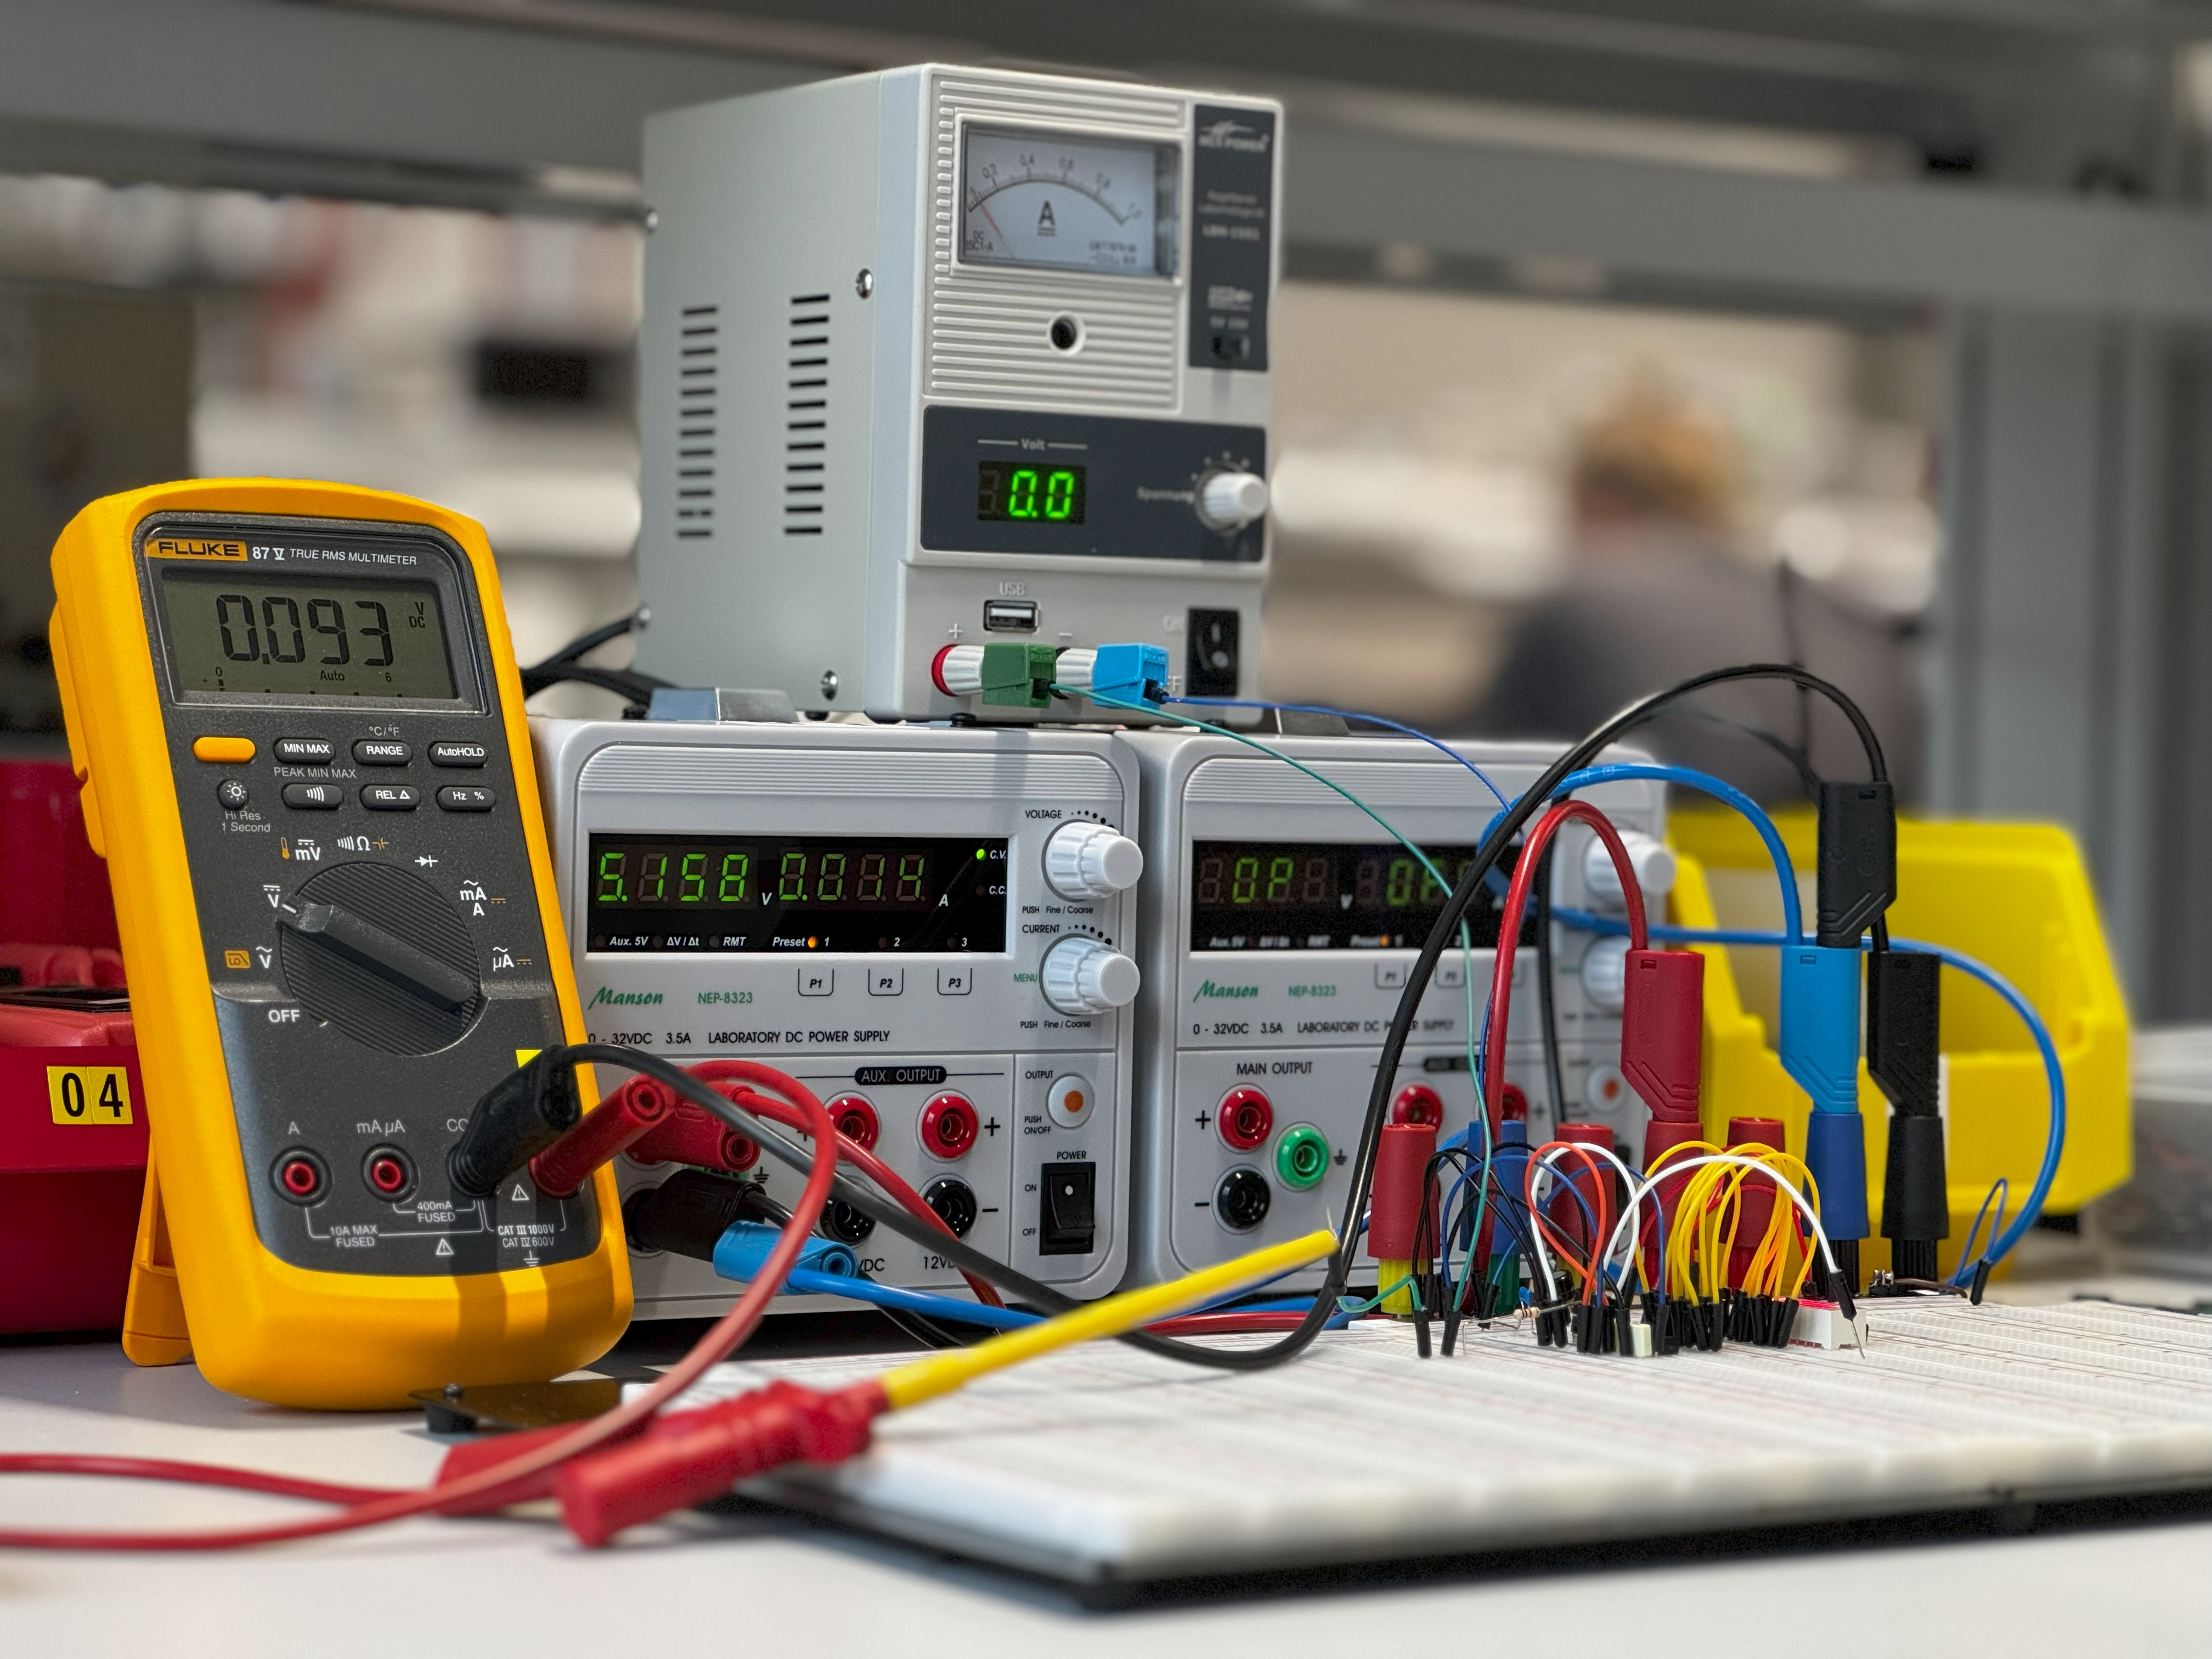
\includegraphics[width=1.0\textwidth]{../Quellen/Labor2/Titelbild.jpg}
\end{figure}
\newpage
\tableofcontents
\newpage

\section*{Einführung und Überblick}
\addcontentsline{toc}{section}{Einführung und Überblick}
Die moderne Messtechnik bildet die Grundlage zahlreicher technischer sowie naturwissenschaftlicher Erkenntnisse. Allerdings ist zu berücksichtigen, dass Messergebnisse niemals vollständig fehlerfrei sind. Die Ursachen für Messfehler und -ungenauigkeiten sind vielfältig. Als Ursachen für Messfehler und -ungenauigkeiten können beispielsweise eine fehlende Kalibrierung, Linearität und Stabilität der verwendeten Messinstrumente oder eine mangelnde Qualität des Messobjekts genannt werden. Des Weiteren kann auch der*die Messende selbst als Ursache in Betracht gezogen werden, welcher, zum Beispiel durch eine mögliche Sehschwäche oder einen ungünstigen Winkel, die Messwerte ungenau abliest. Nicht angepasste oder unvollkommene Messmethoden können ebenfalls zu einer Verfälschung der Messung führen.\\
Genannte Ursachen können zu drei verschiedenen Fehlerarten führen: grobe, statistische und systematische Fehler. \\

\noindent In diesem Laborbericht werden Versuche beschrieben, welche die Genauigkeit verschiedener Bauteile ermitteln. Des Weiteren beschäftigen sich diese mit Fehlerrechnung



\newpage

\section{Versuch 1: Kapazitätsmessung eines unbekannten Kondensators (Black Box)}

\subsection{Zielsetzung}
Das Ziel des ersten Versuchs bestand darin, die Kapazität eines unbekannten Kondesators in einer Black-Box zu bestimmen. 

\subsection{Bauteile und Messgeräte}
\subsubsection*{Messgeräte}
\begin{itemize}
\item Teledyne Technologies Funktionsgenerator T3AFG80 80 MHz
\item Keysight Oszilloskop (DSOX1102A)
\item Fluke 87 V True RMS Multimeter
\item Oszilloskop BNC Tastkopf mit Messeklemme
\item Steckkabel (mehrere)
\item Tru Components Steckbrett
\item Bananenkabel (schwarz und rot)
\item Sicherheits-Klemmprüfspitze (2 Stück)
\end{itemize}

\subsubsection*{Bauteile}
\begin{itemize}
\item Black-Box (Nr. 18-30)
\item Widerstand Nominalwert 4,7 k$\Omega$
\end{itemize}
\newpage

\subsection{Messkonzept}
Zu Beginn wurde die Formel der Ladekurve \( u\textsubscript{c} = U (1 -e ^{-\frac{t}{RC}}) \) und der Entladekurve  \( u\textsubscript{c} = Ue ^{-\frac{t}{RC}}) \) grafisch am Computer dargestellt (siehe Figure 1). 

\begin{figure}[H]
    \centering
    \includegraphics[width=1.0\textwidth]{../Quellen/Labor2/Lade-EntladefunktionSkizze.png}
\caption{Ladekurve (blau) und Entladekurve (rot) eines Kondensators}
\end{figure}

\noindent Diese sollte in den folgenden Schritten mit dem Oszilloskop sichtbar gemacht werden. Hierzu wurde der Funktionsgenerator wie in Table 1 notiert eingestellt.

\begin{table}[H]
	\centering
	\begin{tabular}{|c|c|c|c|}
		\hline
		\textbf{Frequenz} & \textbf{Signalform} & \textbf{Amplitude} & \textbf{Offset}\\
		\hline
		500 Hz & Rechtecksignal & 5 V\textsubscript{pp} & 2.5 V\textsubscript{dc}\\
		\hline
	\end{tabular}
	\caption{Einstellungen des Funktionsgenerators}
\end{table}



\subsection{Messergebnisse}
\begin{table}[H]
	\centering
	\scalebox{0.8}{	
\begin{tabular}{|c|c|c|c|c|c|}
		\hline
		\textbf{Fehlerquelle} & \textbf{Einfluss} & \textbf{typische Größe} & \textbf{stat. oder sys.} & \textbf{Berücksichtigung?} & \textbf{relevant?}\\
		\hline
		R = 4.7 k$\Omega$ & DMM-Messung & \textperthousand ~siehe Datenblatt & statistisch & Fehlerrechnung & Ja\\
		\hline
		Oszilloskop & R\textsubscript{i},C\textsubscript{i} Tastkopf (10x) & 10 µ$\Omega$, $\sim$pF & systematisch & Nein \( < 0.5 \)\textperthousand & Nein\\
		  & x, y - Messung & \(\approx 3\) \% Datenblatt! & statistisch & Fehlerrechnung & Ja\\
		  & Curser & Steigung beachten & statistisch & Fehlerrechnung & Ja\\
		\hline
		Funktionsgenerator & Anstiegszeit & einige ns & systematisch & \( \approx 1 \) \textperthousand & Nein\\
		  & R\textsubscript{i} & 50 $\Omega$ & systematisch & Korrektur & Ja\\
		  &   & $\Delta R$\textsubscript{i} (\(\approx 1\)\%) & statistisch & 1$\%$ \( \Rightarrow\) $\pm ~0.5~\Omega$ & Nein\\
		  & Amplitude, Offset & - & systematisch & relativ & Nein\\
		\hline
		Kabel +5 V & Widerstand & \(\approx 20\)m$\Omega$ & systematisch & zu klein & Nein\\
		\hline
	\end{tabular}
	}
	\caption{...}
\end{table}



\section{Versuch 2: Passiver Zweipol (Black Box)}
\subsection{Zielsetzung}
Bestimmung der Bauteile Typen (Möglichkeiten: R, L oder C) und deren Anordnung innerhalb einer
Black Box.

\subsection{Bauteile und Messgeräte}
\begin{itemize}
\item Netzgerät (NEP-8323)
\item Fluke 87 V True RMS Multimeter
\item Keysight Oszilloskop (DSOX1102A)
\item Bananenkabel (mehrere: rot, blau, schwarz)
\item Sicherheits-Klemmprüfspitze (2 Stück)
\item Oszilloskop BNC Tastkopf mit Messeklemme
\item Steckkabel (mehrere: im Idealfall verschiedene Farben)
\item Steckbrett\\
\end{itemize}


\begin{itemize}
\item A/D Converter - ADC080x
\item 10 Segment LED-Bar - OSX10201-B
\newpage
\item Kondensatoren: 
	\begin{itemize}
	\item 10 µF "Tantalum"
	\item 0,1 µF (2 Stück)
	\item 150 pF
	\end{itemize}
\item Widerstände: 
	\begin{itemize}
	\item 1k$\Omega$
	\item 10k$\Omega$
	\item 8 x 1 k$\Omega$ Widerstandsnetzwerk
	\end{itemize}
\end{itemize}

\subsection{Messkonzept}
...

\begin{figure}[H]
    \centering
   % \includegraphics[]{}
\caption{...}
\end{figure}


\subsection{Messergebnisse}
...

\section{Versuch 3: Leistungsaufnahme eines elektrischen Widerstands}
\subsection{Zielsetzung}
Es soll die elektrische Leistung bestimmt werden, die bei Stromdurchfluss in
einem Widerstand R anfällt.

\subsection{Bauteile und Messgeräte}
\begin{itemize}
\item Netzgerät (NEP-8323)
\item Fluke 87 V True RMS Multimeter
\item Keysight Oszilloskop (DSOX1102A)
\item Bananenkabel (mehrere: rot, blau, schwarz)
\item Sicherheits-Klemmprüfspitze (2 Stück)
\item Oszilloskop BNC Tastkopf mit Messeklemme
\item Steckkabel (mehrere: im Idealfall verschiedene Farben)
\item Steckbrett\\
\end{itemize}


\begin{itemize}
\item A/D Converter - ADC080x
\item 10 Segment LED-Bar - OSX10201-B
\newpage
\item Kondensatoren: 
	\begin{itemize}
	\item 10 µF "Tantalum"
	\item 0,1 µF (2 Stück)
	\item 150 pF
	\end{itemize}
\item Widerstände: 
	\begin{itemize}
	\item 1k$\Omega$
	\item 10k$\Omega$
	\item 8 x 1 k$\Omega$ Widerstandsnetzwerk
	\end{itemize}
\end{itemize}

\subsection{Messkonzept}
...

\begin{figure}[H]
    \centering
   % \includegraphics[]{}
\caption{...}
\end{figure}


\subsection{Messergebnisse}
...

\section{Versuch 4: Widerstandsmessung mittels Vierdrahtmethode}
\subsection{Zielsetzung}
Es soll der (sehr niederohmige) Übergangswiderstand eines Kabels inclusive seiner Steckverbinder
mittels der Vierdrahtmethode gemessen werden.

\subsection{Bauteile und Messgeräte}
\begin{itemize}
\item Netzgerät (NEP-8323)
\item Fluke 87 V True RMS Multimeter
\item Keysight Oszilloskop (DSOX1102A)
\item Bananenkabel (mehrere: rot, blau, schwarz)
\item Sicherheits-Klemmprüfspitze (2 Stück)
\item Oszilloskop BNC Tastkopf mit Messeklemme
\item Steckkabel (mehrere: im Idealfall verschiedene Farben)
\item Steckbrett\\
\end{itemize}


\begin{itemize}
\item A/D Converter - ADC080x
\item 10 Segment LED-Bar - OSX10201-B
\newpage
\item Kondensatoren: 
	\begin{itemize}
	\item 10 µF "Tantalum"
	\item 0,1 µF (2 Stück)
	\item 150 pF
	\end{itemize}
\item Widerstände: 
	\begin{itemize}
	\item 1k$\Omega$
	\item 10k$\Omega$
	\item 8 x 1 k$\Omega$ Widerstandsnetzwerk
	\end{itemize}
\end{itemize}

\subsection{Messkonzept}
...

\begin{figure}[H]
    \centering
   % \includegraphics[]{}
\caption{...}
\end{figure}


\subsection{Messergebnisse}
...


\section{Versuch 5: Statistik}
\subsection{Zielsetzung}
Bestimmung einer gemessenen Zufallsverteilung und ihrer Eigenschaften (Momente). Hierbei stellt
das vorgegebene Los von Widerständen eine willkürlich entnommene Stichprobe einer vom
Hersteller erzeugten Grundgesamtheit dar.


\subsection{Bauteile und Messgeräte}
\begin{itemize}
\item Netzgerät (NEP-8323)
\item Fluke 87 V True RMS Multimeter
\item Keysight Oszilloskop (DSOX1102A)
\item Bananenkabel (mehrere: rot, blau, schwarz)
\item Sicherheits-Klemmprüfspitze (2 Stück)
\item Oszilloskop BNC Tastkopf mit Messeklemme
\item Steckkabel (mehrere: im Idealfall verschiedene Farben)
\item Steckbrett\\
\end{itemize}


\begin{itemize}
\item A/D Converter - ADC080x
\item 10 Segment LED-Bar - OSX10201-B
\newpage
\item Kondensatoren: 
	\begin{itemize}
	\item 10 µF "Tantalum"
	\item 0,1 µF (2 Stück)
	\item 150 pF
	\end{itemize}
\item Widerstände: 
	\begin{itemize}
	\item 1k$\Omega$
	\item 10k$\Omega$
	\item 8 x 1 k$\Omega$ Widerstandsnetzwerk
	\end{itemize}
\end{itemize}

\subsection{Messkonzept}
...

\begin{figure}[H]
    \centering
    %\includegraphics[]{}
\caption{...}
\end{figure}


\subsection{Messergebnisse}
\begin{table}[H]
	\centering
	\begin{tabular}{|c|c|c|c|}
		\hline
		Widerstand & Wert in k$\Omega$ & Widerstand & Wert in kOhm \\
		\hline
		1 & 1.183 & 14 & 1.183 \\
		2 & 1.181 & 15 & 1.180 \\
		3 & 1.186 & 16 & 1.183 \\
		4 & 1.181 & 17 & 1.180 \\
		5 & 1.186 & 18 & 1.182 \\
		6 & 1.183 & 19 & 1.184 \\
		7 & 1.182 & 20 & 1.183 \\
		8 & 1.181 & 21 & 1.184 \\
		9 & 1.187 & 22 & 1.187 \\
		10 & 1.181 & 23 & 1.182 \\
		11 & 1.188 & 24 & 1.179 \\
		12 & 1.186 & 25 & 1.187 \\
		13 & 1.179 & - & - \\
		\hline
	\end{tabular}
	\caption{...}
\end{table}

\section{Versuch 6: Aktiver Tiefpass erster Ordnung}
\subsection{Zielsetzung}
Bestimmung der frequenzabhängigen Verstärkung eines aktiven Tiefpasses

\subsection{Bauteile und Messgeräte}
\begin{itemize}
\item Netzgerät (NEP-8323)
\item Fluke 87 V True RMS Multimeter
\item Keysight Oszilloskop (DSOX1102A)
\item Bananenkabel (mehrere: rot, blau, schwarz)
\item Sicherheits-Klemmprüfspitze (2 Stück)
\item Oszilloskop BNC Tastkopf mit Messeklemme
\item Steckkabel (mehrere: im Idealfall verschiedene Farben)
\item Steckbrett\\
\end{itemize}


\begin{itemize}
\item A/D Converter - ADC080x
\item 10 Segment LED-Bar - OSX10201-B
\newpage
\item Kondensatoren: 
	\begin{itemize}
	\item 10 µF "Tantalum"
	\item 0,1 µF (2 Stück)
	\item 150 pF
	\end{itemize}
\item Widerstände: 
	\begin{itemize}
	\item 1k$\Omega$
	\item 10k$\Omega$
	\item 8 x 1 k$\Omega$ Widerstandsnetzwerk
	\end{itemize}
\end{itemize}

\subsection{Messkonzept}
...

\begin{figure}[H]
    \centering
 %   \includegraphics[]{}
\caption{...}
\end{figure}


\subsection{Messergebnisse}
...




\section{Diskussion}
Was würden Sie nächstes Mal anders machen? Was hat besondere Schwierigkeiten bereitet?

\end{document}
